\documentclass[letterpaper,twocolumn,10pt]{article}

\usepackage{graphicx}
\usepackage{url}
\usepackage[toc,page]{appendix}
%\usepackage{winfonts}

\makeatletter
\newcommand\appendix@section[1]{%
  \refstepcounter{section}%
  \orig@section*{Appendix \@Alph\c@section: #1}%
  \addcontentsline{toc}{section}{Appendix \@Alph\c@section: #1}%
}
\let\orig@section\section
\g@addto@macro\appendix{\let\section\appendix@section}
\makeatother

% Hi Everyone, we can start with this template Cynthia gave us and go from here
% The comment feature is great for annotating text, use it!
% pdflatex should compile this just fine for now

% This file will be the main file, I just splitted the sections in different latex files, so we can modify any section in an easy and simple way. I joined all the sections in the paper using the \input{filename} command.
\begin{document}

\title{AuditBear}
\author{David Wagner
\and Cynthia Sturton
\and Annie Edmundson
\and Keishla Ortiz
\and Ana Maria Quevedo
\and Samuel Rodriguez
\and Patrick Baxter}
% Add additional authors:
% \and Author n
\maketitle

%Abstract

%Changes here (in the main paper I'll just invoke this file)
\subsection*{Abstract}
Voting audit logs, produced by electronic voting systems, contain information that is useful for uncovering procedural errors and election anomalies, but are currently unwieldy and hard for election officials to use in post-election audits.  We have devised a way to make the auditing process quick and efficient for election officials.  In order to audit elections, we develop new techniques for detecting equipment problems and procedural mistakes made by election workers; we have automated these analyses for a user-friendly process.  We implemented our methods and built a website for this tool that has the capability of analyzing electronic voting machine log files.  We intend for this work to assist those working with election auditing to quickly identify voting equipment or procedural issues and correct them before election results are certified.  Such issues include locating voting machines or media containing vote data that have not been included in the aggregated count, and voting equipment that needs maintenance before the next election.

%Introduction section
\bigvertspace
\section{Introduction}
\smvertspace
A DRE is a type of electronic voting machine in which the
voter interacts directly with the machine, typically through a touch
screen. DREs provide a friendly interface to assist the voter with the
ballot marking process. Similar to the commonly used optical scan
systems, DRE units can reduce overvoting and undervoting. Uniquely,
DRE machines can issue electronic ballots on demand; running out of
paper ballots is no longer an issue. Additionally, audio DREs can
assist visually impaired voters.
 
Federal standards require that electronic voting machines generate
detailed audit logs, which can be used during post-election
audits. These logs record events as they occur on the voting machine 
such as opening the machine for voting, casting a vote or closing the
machine at the end of election day. The log data may also include a
record of every ballot cast in the voting machine.  Previous work has
shown how these logs can be analyzed to uncover procedural errors and
anomalies that occur during the election\cite{Buell2011}.
Unfortunately, manual analysis of raw log data is usually cumbersome
and time consuming, making county-wide post-election analysis
impractical and prone to human error. Therefore, at the present time,
election officials do not regularly perform these types of analyses. 

We aim to make DRE audit log analysis more useful and accessible to
both election officials and other interested parties. In this work, we
develop new methods to analyze these audit logs for the detection of
both procedural errors and system deficiencies. We created a public
web application that applies our methods to detect procedural errors
and system deficiencies.  Election officials can use our tool to
identify memory cartridges containing precinct totals that were not
uploaded on election night, machines that may have experienced
hardware problems during the election, and polling locations that
closed late or had voters waiting in line for extended periods.
 
Our research builds on a similar study that was conducted with DRE audit data collected by fourteen South Carolina counties during the 2010 primary and general elections.  The authors of that study were able to determine, solely by analyzing the audit logs, that 1127 votes did not get included in the official certified tally in Richland County, South Carolina~\cite{Buell2011}. These findings were possible because DRE systems used in South Carolina produce three different types of audit logs, each capturing slightly different information. By cross checking the logs against each other, the authors found inconsistencies that enabled them to uncover the missing votes. In our research we used the same data set as a basis for development of our software. First, we replicated the detection of votes not uploaded. We took this matter further and found fifteen memory devices containing votes that were not uploaded to the tabulation systems from seven counties during the 2010 General election. These memory devices tallied 2082 total votes. Without additional information we could not verify if alternate procedures were used to add these missing votes to the aggregated totals. 

We implement these methods for the ES\&S iVotronic DRE as the 2010 South
Carolina data was already publically available through a previous
Freedom of Information Act request and the iVotronic was used in that election. \cks{Is this true? I changed the wording, but I'm not actually sure
  how the data was made available.} The iVotronic system is a
standalone, portable, touchscreen system that records vote totals,
ballot images and an event log on internal flash 
memory. The event log records, in chronological order, the system
events including unit configuration, polls opened, votes cast, polls
closed, calibration or battery issues, and system errors or warnings. 
iVotronic voting machines represent one of the most widely deployed
DREs in the U.S. In 2010, 422 jurisdictions tallying more than 22
million registered voters used this system~\cite{VerVot2010}. However, our methods for analysis of audit logs
are applicable to all DRE voting systems  that produce the necessary
audit logs.  

A brief description of several problems we detect follows.

\textbf{Votes not uploaded.} We detect  memory cartridges used to close voting machines that have not had their vote data uploaded to the tabulation system. This situation, if not corrected, can result in votes left out of the official results.

\textbf{Machines not closed.} We detect voting machines that were not
closed for voting at the polling location. Failure to close a machine
on election night may result in its votes being left out of the
certified count.

\textbf{Missing terminals from the audit database.} This analysis
identifies voting machines used during the election whose event log or
ballot images have not been uploaded to the election reporting
software. Complete DRE ballot images and event logs will allow for
more accurate post-election audits. 

\textbf{Polling location related analyses.} Our tool provides a series of analyses related to polling location activity. We identify locations that stayed open late as well as locations that may have experienced long lines during the day. This information can help county officials to identify locations that may need additional resources in the future. 

\textbf{DRE voting machine configuration and hardware problems.} Our tool performs several analyses that can identify  voting machines that may need testing, repair or reconfiguration. These analyses include identifying possible calibration issues, machines with potential power supply issues, machines that were forced to close early, and machines with incorrect date and time settings.

\textbf{Poll worker training related issues.} We also identify incorrect procedures at the precincts such as using the wrong cartridge to close the voting machines in a precinct, forgetting to print the precinct's zero tape or activating ballots with the incorrect cartridge. Election officials may be able to use this information to improve poll worker training and minimize recurrences in the future.

In this work we assume that DRE audit logs are complete, accurate,  trustworthy, and free of accidental or malicious tampering. Detecting and preventing audit log tampering is outside of the scope of this work.

In summary, this paper develops and implements new ways that audit log data can be used meaningfully and in an automated fashion to enhance the accuracy and efficiency of elections. We believe our tool will provide useful feedback to election administrators during the canvassing process. We hope that this study illustrates the potential value of voting systems' audit logs and motivates future election technologies to provide enhanced support for these purposes.




%Background section
\section{Background}

\subsection{Introduction to the iVotronic}
Approximately 422 jurisdictions in the United States used the ES\&S iVotronic electronic voting terminal in 2010.  A brief description of  its functionality and main system components follows:

\begin{itemize} 
\item Voting terminal. The voting terminal is a stand-alone touchscreen voting  unit. The ports available in the back of the terminal include: serial port, compact flash card slot and power supply port. The terminal is equipped with an internal battery which keeps the terminal operational during power failure periods. To comply with federal standards, at least one audio (ADA) terminal is placed in each precinct to assist the visually impaired voters.

\item Personalized Electronic Ballot (PEB). The PEB is a proprietary cartridge designed by ES\&S to operate the iVotronic terminal.  The PEB is placed in a slot located to the left of iVotronic\textquoteright s touchscreen. The terminal and the PEB communicate through the infrared port. The South Carolina counties deploy two types of PEBs to the precinct: a) the green band master PEB and b) the red band activator PEB. Both types of PEB have the same functionality, however, poll workers are trained to perform the following tasks with each PEB type.
    \begin{itemize}
    \item Master PEB.  Poll workers use the master PEB to open polls on election day. When the PEB is placed in the terminal, the touchscreen displays the precinct\textquoteright s name programmed in the PEB so that poll workers can verify the polling location information and date/time registered in the terminal\textquoteright s internal clock. If the information displayed is correct, the poll workers open the terminal for voting. The same master PEB should be used to open all terminals of the polling location. In the same fashion, the master PEB should be used to close all terminals of the polling location at the end of the voting day. When the terminal closes, it uploads  its totals onto the master PEB. The master PEB accumulates the precinct totals which are accumulated into the official tally.
    \item Activator PEB.  This PEB is used by  poll workers to activate ballots for voters. The number of activator PEBs that the election officials program for each precinct is proportional to the number of terminals and poll workers assigned to the precinct. The ratio varies depending on the jurisdiction criteria.
    \end{itemize}
\item Removable Compact Flash card (CF). The CF cards are programmed at election central and installed in the back of the voting terminal prior to precinct deployment. The CF cards contains graphic (bitmap) files read by the voting terminal during the voting process. The CF cards are also used as an external memory device: the audit log and ballot images are written to the CF card when the terminal is closed for voting. Once the polls close, the CF cards are removed from the back of the terminal and delivered to election headquarters on election night. 

\item External printer module. This module is connected to the serial port on the back of the voting terminal. The thermal printer produces the precinct zero tape and results tape. Poll workers are instructed to print the zero tape once all iVotronics of the precinct are opened for voting. In the same fashion, the results tape should be produced when all voting terminals are closed for voting on election night.
\end{itemize}

\subsection{Description of logs}
We used three iVotronic system logs to perform the analyses described in the next section. The event log (EL152.lst), ballot image file (EL155.lst) and the ES\&S election reporting manager system log (EL168a.lst).  The header of the log files identify the County's name, the type and date of the election, the date the report was generated and the election ID. The election ID is a parameter generated by the ES\&S election programming software to uniquely identify the specific election.

The event log (152.lst) lists all iVotronic terminals used on the election. The log records the terminal configuration at headquarters prior to precinct deployment which begins with the \textquotedblleft clear and test\textquotedblright of the terminal to delete previous election data from the terminal\textquoteright s memory. The log also records, in a chronological order, all relevant election day events including polls open and polls closing and the number of ballots cast.  The event log contains several columns which include: iVotronic's terminal serial number, PEB serial number, PEB type, date, time, event code and event description. An excerpt of  an event log is given in the appendix~\ref{app:el}.

The ballot image file (155.lst) contains all ballot images saved by the iVotronic terminals during the voting process. The ballot images are segregated by precinct and terminal where the votes were cast. The ballots are saved in a random order to protect the privacy of the voter. An asterisk (*) indicates the beginning of each ballot. An excerpt of a ballot image file is given in the appendix~\ref{app:bi}.

The system log listing file (EL168a.lst) tracks activity in the election reporting database since its creation at the election headquarters. Its chronological entries reflect the commands executed by the operator(s) during  pre-election testing, election night reporting and post-election canvassing. This log contains the totals accumulated in the various precincts during election night reporting, as well as any warnings or errors reported by the reporting software system during the tabulation process. The system log also tracks the uploading of the PEBs and CF cards to the central election reporting database. Manual adjustment of precinct totals are also documented in the system log file. An excerpt of a system log file is given in the appendix~\ref{app:sl}.

% Related Work section
\section{Related Work}
Many election technology systems provide a means of auditing elections. For example, in optical scanning systems the cast ballots themselves form a paper record of the votes cast on election day. On the other hand, DRE machines do not provide this type of paper trail. Some DREs provide a Voter Verified Paper Audit Trail (VVPAT), which stores a hard copy version of each ballot cast.  A third type of audit trail, which is produced by all DREs, are the event logs stored electronically on each DRE.  In this section we discuss related work on the analysis of audit logs for post-election auditing. 

Two recent studies used event logs from the iVotronic voting system to audit elections~\cite{Buell2011,Sandler2007}. The authors of the first study~\cite{Buell2011} performed an audit of the same South Carolina elections that we analyzed. Using these audit logs, they discovered votes not included in the certified counts and problems with the audit data. They crosschecked the event log, the ballot images file, and the system log to identify unsupported votes and missing audit data.  By consulting additional audit materials, such as the printed results tapes, the authors were able to offer possible reasons and explanations as to why the problems occurred. Our work takes a slightly different approach.  We focus on developing a variety of methods to analyze the data; in addition, we automate these analyses in order for their use by election officials.  While our tool did discover and report these same problems, we simply report what was wrong, but can not provide a possible explanation for the cause of the error. 

The authors of the second study~\cite{Sandler2007} provided an analysis of vote tallies using the protected count of votes on each machine and comparing this to the printed results tapes. Their report also finds dates that were most likely inaccurate.  With further investigation, they concluded that the hardware clock was incorrect. Our research provides analyses to identify similar problems, but in a way that could be automated. 

There has also been research on using the audit logs to analyze election-day procedure and activity. For example, one recent publication showed how event logs could be used to determine if a machine acted \textquotedblleft normally\textquotedblright on election day~\cite{Antonyan2009}. The authors of this research studied the event logs of the AccuVote Optical Scanning system and used those logs to build a finite state machine that models the sequences of events a well-behaved machine might produce. This type of analysis would be useful to provide for the iVotronic systems that we studied. However, the AccuVote machines have considerably fewer possible event types than the iVotronics so the analysis would become considerably more complex. 

A common problem on election day, which we try to identify in our analysis, is the occurrence of long lines. Many studies have researched ways to mitigate long lines at polling locations ~\cite{Allen2006,Dow2007,Spencer2010,Wilson2008}.  One such study has simulated the flow of voters through the voting process~\cite{Edel2010}. The authors use this simulation to determine the optimal number of voters per voting machine, and correspondingly, the appropriate number of voting machines per polling location based on the number of registered voters at that particular location. Their work is predictive: the authors make some assumptions, such as the average time it takes to vote and when peak voting hours will occur, and use those as a basis for predicting where long lines are likely to occur. Our analysis is descriptive: given the audit logs from election day, we infer the average time it took to vote and use that information to determine whether a particular polling location experienced long lines or not. The two methods are complementary. Predictive models can be used to prevent long lines, while descriptive models can be used to check and refine the prediction algorithms. 

Voter Verified Paper Audit Trails (VVPATs) are a different type of audit log. Unlike the audit logs we used in our analyses, VVPATs are viewed and verified by the voter and are more suited to audits concerning a DRE incorrectly capturing a voter\textquoteright s intent. Our work is more concerned with identifying cases of cast votes not being included in the final count, or issues at the polling place that might prevent the voter from casting their vote in the first place. With VVPATs, as long as a certain percentage of voters do check their paper ballot~\cite{Hall2006}, the voting machine need not be assumed correct, whereas our analyses do make this assumption.

%Conclusion
\section{Conclusion}
We recommend that election administrators conduct routine reviews of the audit logs generated by the voting machines as they contain useful information that can shed light on procedural and election equipment issues. This paper develops methods to analyze audit data from DRE voting machines intended to assist those working with election auditing and integrity.   We perform a variety of analyses on the DRE audit data to detect possible miscounts, procedural errors, voting machine malfunctions, or system deficiencies. With this information, election officials can improve poll worker training, election official checklists, election tabulation procedures, and voting machine preparation testing.

We built a web application to perform these analyses. Election officials just need to upload the DRE log files to our website and run the analyses. By automating our analyses we can provide intelligent feedback to election officials during the canvassing process and help them quickly correct any problems in order to produce accurate election results. These analyses are freely available online at www.audit-bear.org.

%Acknowledgements section
\section{Acknowledgments}


%This tells latex to use our .bib file
\bibliographystyle{plain}
{\footnotesize
\bibliography{paper}}

%Appendix section
\clearpage
\onecolumn
\begin{center}
\appendix
\section{Event Log File}\label{app:el} 
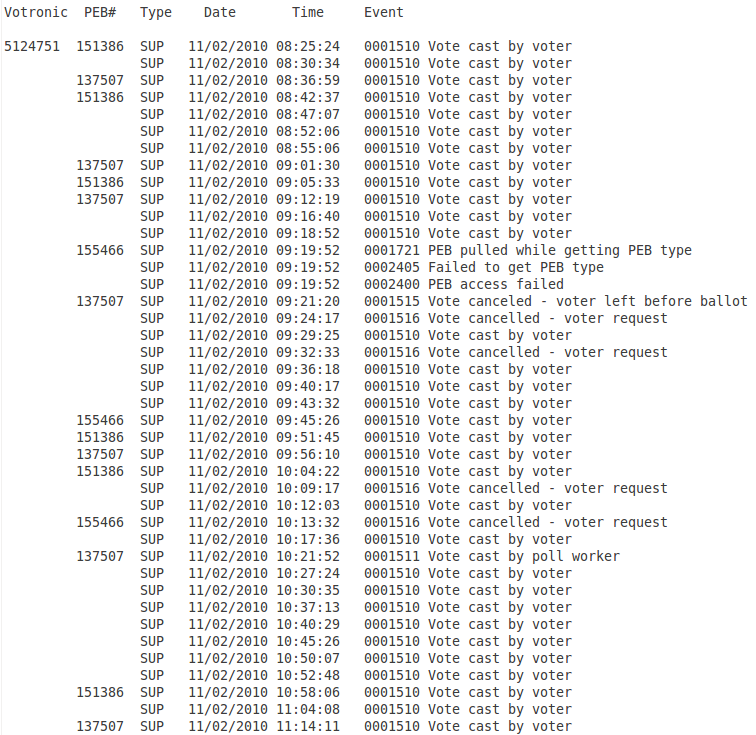
\includegraphics[width=0.8\textwidth]{eventLog}
%~\ref{app:el}

\clearpage
\section{Ballot Image File}\label{app:bi}
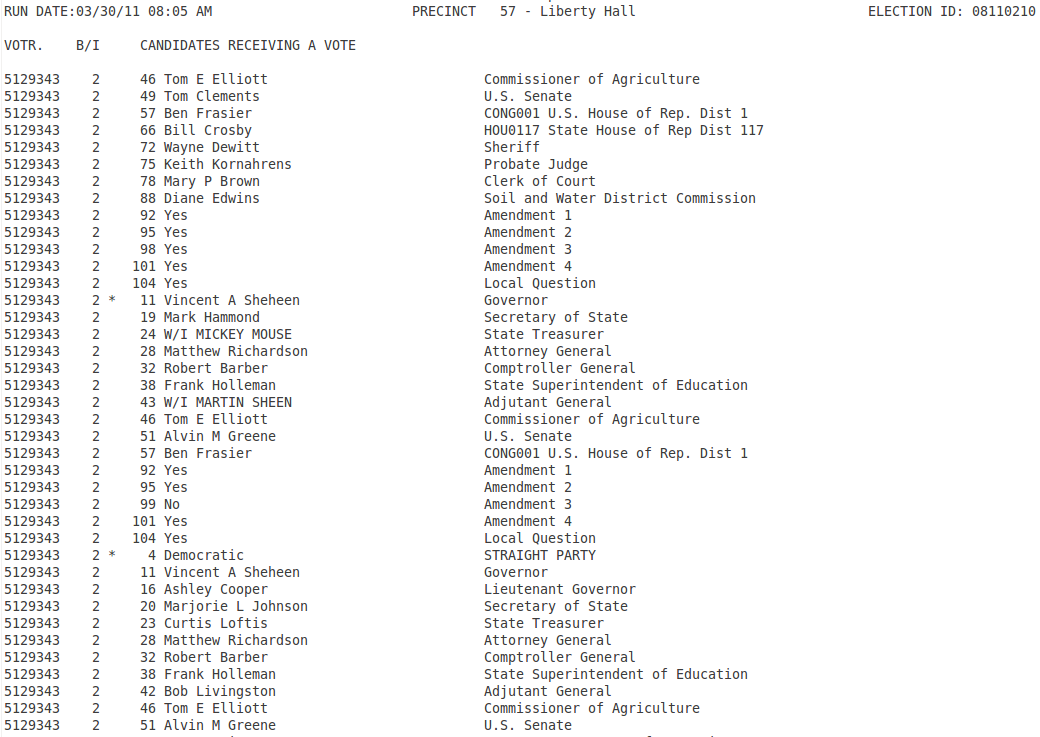
\includegraphics[width=0.9\textwidth]{ballot}
%This is app~\ref{app:bi}

\clearpage
\section{System Log File}\label{app:sl}
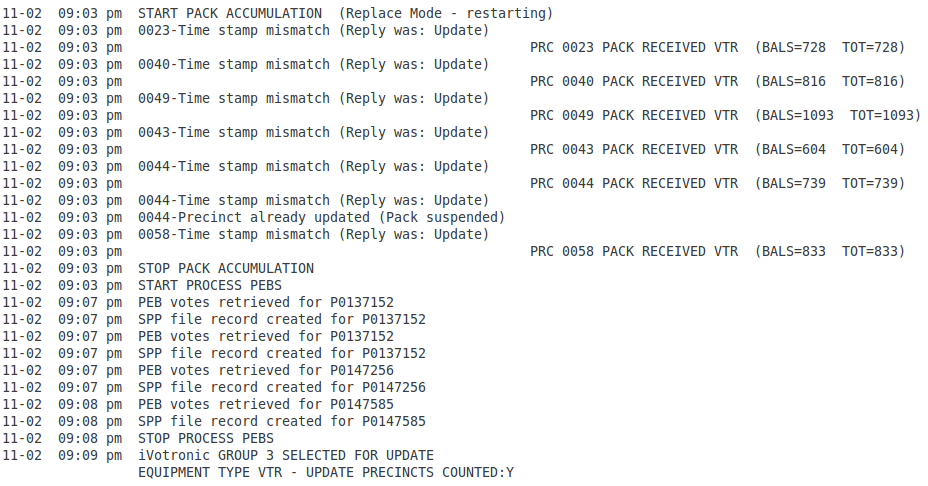
\includegraphics[width=0.9\textwidth]{system}
%This is app~\ref{app:sl}
\end{center}


\end{document}
